%
% The first command in your LaTeX source must be the \documentclass command.
\documentclass[sigplan,screen]{acmart}

%
% defining the \BibTeX command - from Oren Patashnik's original BibTeX documentation.
\def\BibTeX{{\rm B\kern-.05em{\sc i\kern-.025em b}\kern-.08emT\kern-.1667em\lower.7ex\hbox{E}\kern-.125emX}}

% Rights management information.
% This information is sent to you when you complete the rights form.
% These commands have SAMPLE values in them; it is your responsibility as an author to replace
% the commands and values with those provided to you when you complete the rights form.
%
% These commands are for a PROCEEDINGS abstract or paper.
\copyrightyear{2019}
\acmYear{2019}
\setcopyright{acmlicensed}
\acmConference[Mesa '18]{Mesa '18: SER 574}{Jan 20, 2019}{Mesa, AZ}
\acmDOI{11.2222/3333333.4444444}
\acmISBN{111-2-333-4444-1/20/19}

%
% These commands are for a JOURNAL article.
%\setcopyright{acmcopyright}
%\acmJournal{TOG}
%\acmYear{2018}\acmVolume{37}\acmNumber{4}\acmArticle{111}\acmMonth{8}
%\acmDOI{10.1145/1122445.1122456}

%
% Submission ID.
% Use this when submitting an article to a sponsored event. You'll receive a unique submission ID from the organizers
% of the event, and this ID should be used as the parameter to this command.
%\acmSubmissionID{123-A56-BU3}

%
% The majority of ACM publications use numbered citations and references. If you are preparing content for an event
% sponsored by ACM SIGGRAPH, you must use the "author year" style of citations and references. Uncommenting
% the next command will enable that style.
%\citestyle{acmauthoryear}

%
% end of the preamble, start of the body of the document source.
\begin{document}

%
% The "title" command has an optional parameter, allowing the author to define a "short title" to be used in page headers.
\title{Designing an Agile Collaboration: How to Succeed in Cross-Team Interactions}

%
% The "author" command and its associated commands are used to define the authors and their affiliations.
% Of note is the shared affiliation of the first two authors, and the "authornote" and "authornotemark" commands
% used to denote shared contribution to the research.
\author{Paul Horton}
\email{pahorton@asu.edu}
\affiliation{%
  \institution{Arizona State University}
  \city{Mesa}
  \state{Arizona}
  \postcode{85212}
}

\author{Ruby Zhao}
\email{qrzhao@asu.edu}
\affiliation{%
  \institution{Arizona State University}
  \city{Mesa}
  \state{Arizona}
  \postcode{85212}
}

%
% The abstract is a short summary of the work to be presented in the article.
\begin{abstract}
Agile models within the field of software engineering are widely used to facilitate flexibility and ease of communication in order to solve engineering challenges.
For agile teams to succeed on a complex project, they must be able to work not only with their own members but also with other teams.
*****Add a summary of findings******
\end{abstract}

%
% Keywords. The author(s) should pick words that accurately describe the work being
% presented. Separate the keywords with commas.
\keywords{agile, teamwork, design, architecture, project management, software engineering}

%
% A "teaser" image appears between the author and affiliation information and the body
% of the document, and typically spans the page.
% \begin{teaserfigure}
%   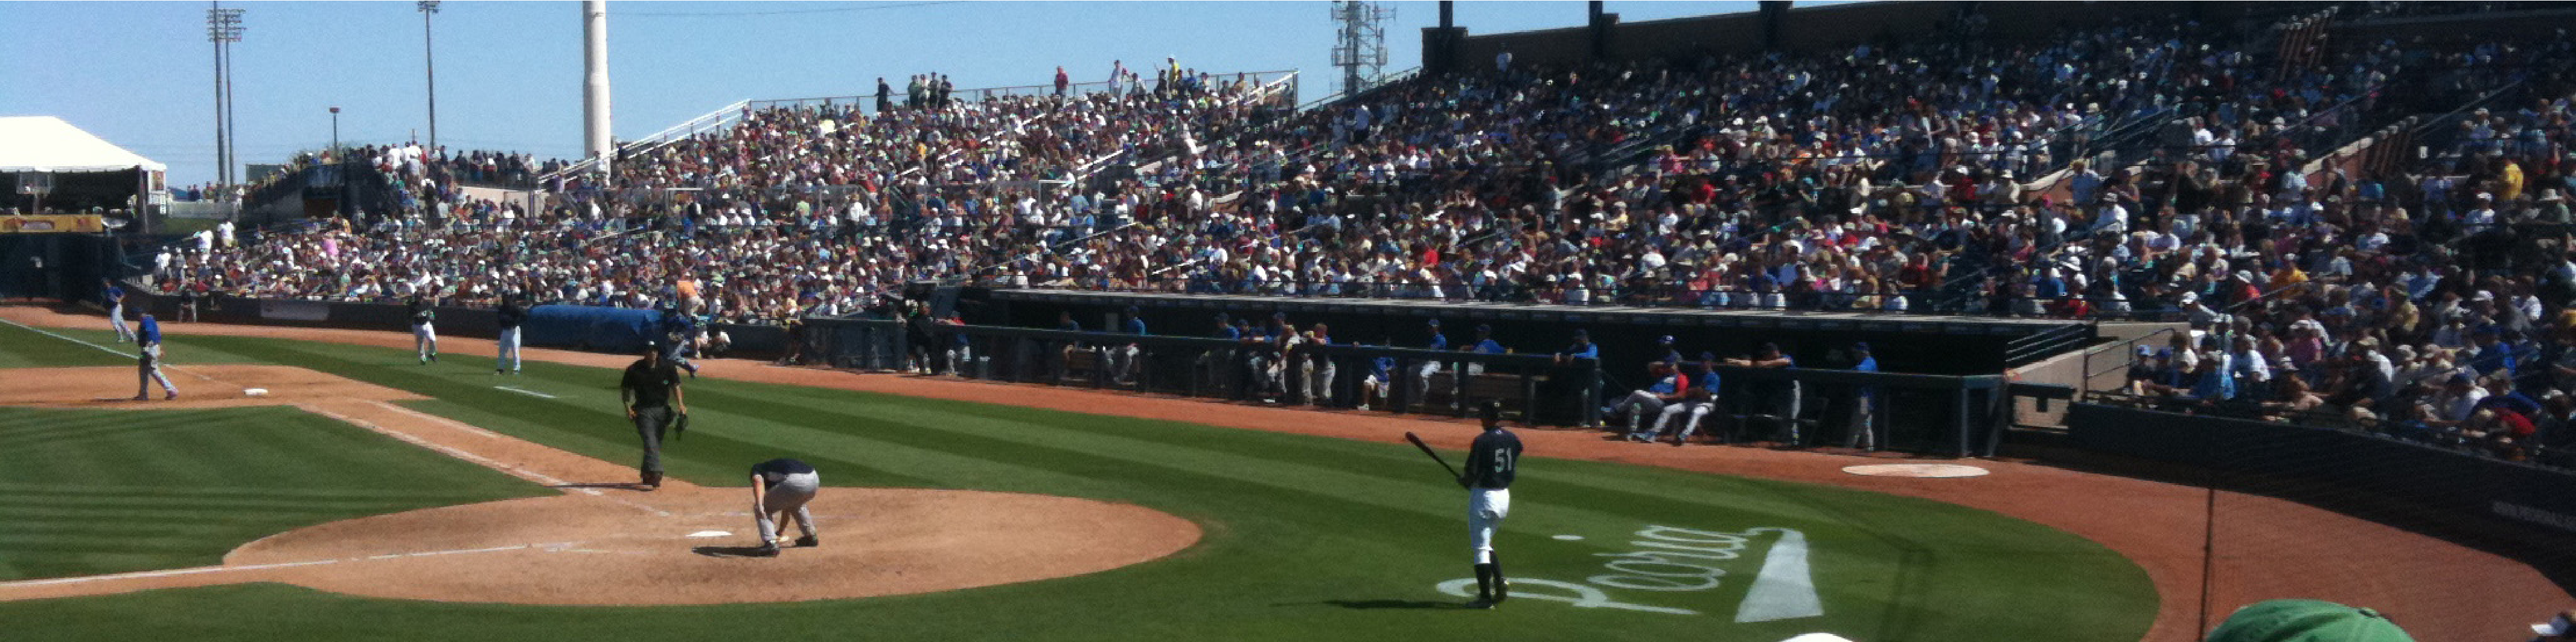
\includegraphics[width=\textwidth]{sampleteaser}
%   \caption{Seattle Mariners at Spring Training, 2010.}
%   \Description{Enjoying the baseball game from the third-base seats. Ichiro Suzuki preparing to bat.}
%   \label{fig:teaser}
% \end{teaserfigure}

%
% This command processes the author and affiliation and title information and builds
% the first part of the formatted document.
\maketitle

\section{Introduction}
Agility is currently the byword of the software engineering field.
Software engineers must respond to customer requirements with speed and flexibility, and for many projects, development teams have turned to Agile methodology as the answer to these demands.
A good agile team is one that communicates, but is also responsive to, changing requirements to and from other teams.
So then, how best should these agile teams communicate with each other, and what tools are at their disposal in order to ensure efficient and accurate communication?
The focus of this paper will be to answer this question of cross-team interaction.
The section "Important Aspects" will discuss which qualities allow teams to work together successfully.
This section lists actionable qualities of a healthy team dynamic that can be incorporated into any team making use of agile processes.
The following section, "Design and Architecture", discusses the role of design and architecture in cross-team communication efforts. Specifically... *****Insert a summary of section 2 here*****

\section{Agile Collaboration}

\subsection{Important Aspects}

\subsection{Design and Architecture}

\section{Conclusion}


%
% The next two lines define the bibliography style to be used, and the bibliography file.
\bibliographystyle{ACM-Reference-Format}
\bibliography{sample-base}


\end{document}
